\section{Aktivitetsmålere til børn} \label{tracker_intro}
\textit{Dette afsnit omhandler optimale egenskaber for en aktivitetsmåler samt funktionaliteten af nuværende aktivitetsmålere til børn. En række nuværende aktivitetsmålere analyseres og vurderes med henblik på at kunne designe en prototype, som opfylder de opstillede succeskriterier.}

\subsection{Aktivitetsmåleres funktionalitet}
Aktivitetsmålere benyttes til at detektere det fysiske aktivitetsniveau hos en bruger. Aktivitetsmålere benytter en eller flere sensorer til at detektere det fysiske aktivitetsniveau. Eksempelvis kan et pedometer, accelerometer eller gyroskop findes i en aktivitetsmåler. Et pedometer bestemmer antal skridt via en svingende pendulhammer i et kredsløb. Et accelerometer måler acceleration i m/s$^2$ eller g-kræfter, hvilket er et udtryk for tyngdepåvirkningen af sensoren under bevægelse. Et gyroskop måler vinkelhastighed i grader per sekund (dps) eller omdrejninger per sekund. Dette kan anvendes til at bestemme orientering eller balanceinformation. \citep{Sparkfun,Woodford2016,Sparkfun_gyro} \newline
Et fælles formål for aktivitetsmålerne er dermed at bestemme de fysiske aktiviteter gennem en række analoge og digitale elementer. De digitale elementer benyttes til at behandle og visualisere sensorens opsamlede data gennem en brugerflade.

\subsection{Succeskriterier for aktivitetsmålere til børn} \label{succeskrav}
Producenter benytter teknologi som et led i at motivere børn til et mere fysisk aktivt liv gennem spil og leg ved hjælp af aktivitetsmålere. \citep{Fuhu2015,PowerAbout2015} En teknologi, som motiverer børn til en aktiv livsstil, vil give samfundsøkonomiske og sundhedsmæssige fordele, idet en aktiv livsstil forbygger diverse følgesygdomme, som beskrevet i \secref{subsec:inover}.

Aktivitetsmålere til børn bør tage højde for en række essentielle kriterier, som blandt andet indebærer en detektering af barnets daglige aktivitet. Aktivitetsmåleren skal dermed detektere og gemme al aktivitet i et barns hverdag i såvel skole- som fritid.\\
Et studie har undersøgt, hvilke børneidrætter der er de 10 mest populære blandt børn i aldersgruppen 7-15 år. Det fremgår af dette studie, at 7 ud af de 10 mest populære børneidrætter involverer gang eller løb \citep{Asserhoej2013}. Desuden fremgår det af flere  studier, at cykling er en af de hyppigst benyttede transportmidler for børn i alderen 10-15 år \citep{DTU2014,COWI2015}. På baggrund af dette vurderes det, at en aktivitetsmåler skal kunne detektere gang, løb og cykling. Dermed registreres størstedelen af et barns samlede fysiske aktivitetsniveau i løbet af en dag. Ydermere bør aktivitetsmåleren kunne skelne mellem aktivitetsformerne, hvilket foregår automatisk igennem genkendelse ved brug af forskellige sensorer. Herved kan aktivitetsmåleren opnå en stor brugervenlighed, idet barnet ikke selv skal indtaste, hvilken type fysisk aktivitet der udføres. \newline
Intensiteten af en given fysisk aktivitet kan bestemmes af en persons puls, som det fremgår i \secref{subsec:fysio_aktivitet}. Det vil være fordelagtigt, at aktivitetsmåleren kan bestemme barnets puls og herigennem kategorisere intensiteten.

Målgruppen for den tilsigtede aktivitetsmåler er børn i aldersgruppen 9-12 år. Det er påvist, at børn i denne aldersgruppe motiveres bedst gennem frivillig fysisk aktivitet med intrinsisk motivation som leg og spil. Aktivitetsmåleren skal derfor kunne benytte sig af en type motivation, som henvender sig til målgruppens behov. \\
Aktivitetsmålerens placering og påmontering skal desuden være komfortabel. Aktivitetsmåleren må ikke fratage eller hindre barnets psykiske eller fysiske udfoldelse i forbindelse med afbenyttelse. 

Den optimale aktivitetsmåler til målgruppen skal dermed kunne: 
\begin{itemize}
\item Detektere gang.
\item Detektere løb.
\item Detektere cykling. %Når de står detekteret hver for sig, så menes der derved, at de kan skelnes fra hinanden.
\item Detektere fysiske aktiviteters intensitet. %igennem puls
\item Motivere fysisk inaktive og aktive børn til et øget fysisk aktivitetsniveau. %socialt
\item Monteres og placeres på komfortabel vis.
\end{itemize}

\subsubsection{Afgrænsning af aktivitetsmålere}  %Hed før Baggrund for analyse og vurdering af aktivitetsmålere
Der er udvalgt fire aktivitetsmålere til videre analyse, som alle har samme formål: at motivere børn til et øget fysisk aktivitetsniveau. De udvalgte aktivitetsmålere henvender sig alle til børn i målgruppen 9-12 år og har på forskellig vis udformet en brugerflade, som er motiverende. Ydermere er aktivitetsmålerne trådløse og tilbyder en brugerflade gennem trådløs overførsel i form af en hjemmeside og/eller applikation (app). \newline
De udvalgte aktivitetsmålere vil blive analyseret og vurderet på baggrund af de opstillede succeskriterier.

\subsection{UNICEF kid power band}
UNICEF Kid Power Band er en aktivitetsmåler, som henvender sig til børn ved at hjælpe børn i ressourcefattige lande, hvoraf sloganet til aktivitetsmåleren lyder: "Vær aktiv. Red liv". Aktivitetsmåleren er udformet som et armbånd, hvilket fremgår af~\figref{fig:unicef}. Aktivitetsmåleren benytter et pedometer og et accelerometer til at detektere barnets fysiske aktivitet. Det opsamlede data overføres trådløst via Bluetooth til en app. \citep{PowerAbout2015,PowerManual2015}
\begin{figure}[H]
	\centering
	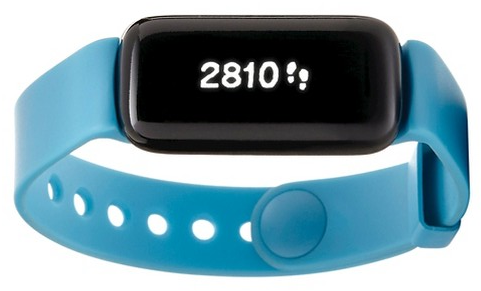
\includegraphics[scale=0.4]{figures/aProblemanalyse/unicef.png}
	\caption{På figuren ses UNICEF kid power band, udformet som et armbånd. \cite{Unicef2016}}
	\label{fig:unicef}
\end{figure}\vspace{-.25cm}
Børnene kan optjene point ved at være fysisk aktive, som omregnes til en sum penge, der sponsoreres af fans, firmaer og forældre. Pengene bliver doneret til ressourcefattige lande, som er en del af UNICEFs tiltag. 
Børnene har mulighed for at vælge mellem en række udvalgte lande gennem missioner. Disse missioner skal lære børnene om samfundet i det pågældende land og giver børnene indsigt i betydningen af deres hjælp. Resultaterne samles i en app, hvor børnene har mulighed for at følge med i progressionen for dem selv samt deres venner samt for de missioner, som de deltager i.~\citep{PowerAbout2015,PowerManual2015}\\
Aktivitetsmåleren har en indkøbspris på 285 kr. \citep{Unicef2016}

\subsubsection{Vurdering af succeskriterier}
Aktivitetsmålerens funktioner vurderes ud fra opstillede succeskriterier i \secref{succeskrav}. \\
Aktivitetsmålerens funktion er at tælle skridt, hvilket detekteres under løb og gang, dog skelnes der ikke mellem aktiviteterne. Da armene ikke bevæges ved cykling, er denne aktivitetsform ikke mulig at detektere. Aktivitetsmåleren kan ikke detektere intensiteten af den målte aktivitet, idet der kun måles på, hvor energisk armen bevæges under en given øvelse. Aktivitetsmåleren er designet som et armbånd med en justerbar rem, hvilket gør at den kan monteres og placeres på komfortabel vis. \citep{PowerManual2015} \newline
Børnene udfører de fysiske aktiviteter sammen med andre børn med henblik på at hjælpe børn i ressourcefattige lande. Aktivitetsmåleren motiverer børnene intrinsisk og ekstrinsisk ved hjælp af de sociale aspekter, som ligger til grund for aktivitetsmålerens brugerflade.~\citep{PowerAbout2015} 

UNICEF Kid Power Band opfylder to ud af seks succeskriterier, mens det delvist opfylder to succeskriterier. En oversigt kan ses i \tabref{tab:sammenhold_tracker}.

\subsection{The Sqord Booster}
The Sqord Booster er en aktivitetsmåler, som appellerer til børn i alderen 8-14 år gennem konkurrence og fællesskab. Aktivitetsmåleren kan placeres om håndleddet som et armbånd, hvilket kan ses på \figref{fig:sqord}. Aktivitetsmålerens chip kan også placeres i en lomme eller bindes til skoen angiveligt uden indflydelse på målingerne, som sensorerne udfører. 
\begin{figure}[H]
	\centering
	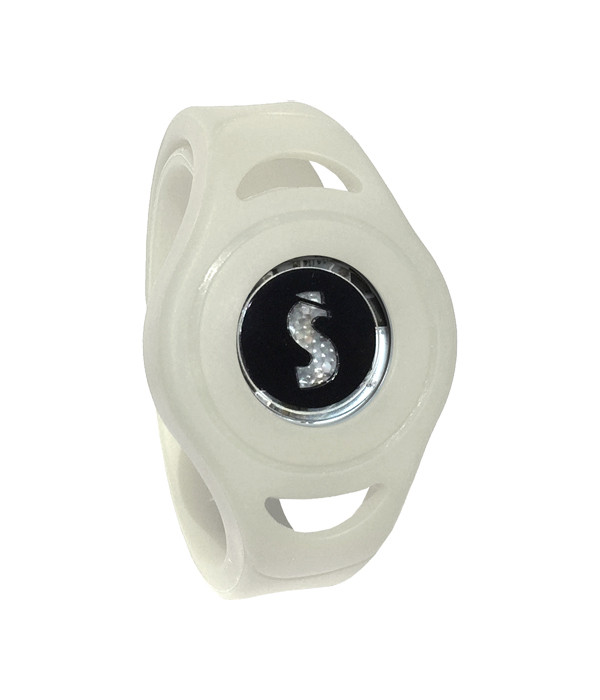
\includegraphics[scale=0.25]{figures/aProblemanalyse/sqord.JPG}
	\caption{På figuren ses The Sqord Booster udformet som et armbånd. \citep{Sqord2016}}
	\label{fig:sqord}
\end{figure}\vspace{-.25cm}
Aktivitetsmåleren motiverer børn igennem spil, hvor alt udført aktivitet gemmes i en avatar. Denne avatar designer børnene selv på en hjemmeside, hvor de også kan kommunikere med deres venner. Forældrene har mulighed for at oprette et forældrelogin til siden, så de ligeledes kan følge med i barnets aktivitet. Aktivitetsmåleren er designet til at blive brugt i grupper men er ikke betinget af fysisk tilstedeværelse, da online gruppekommunikation også er muligt. Børnene kan enten konkurrere mod hinanden eller arbejde sammen som et hold. Det er også muligt at benytte aktivitetsmåleren individuelt, da barnet kan følge egen og andres udvikling. Hermed kan der opstå interne konkurrencer i forbindelse med barnets formåen. \citep{Sqord_family2015,Sqord_group2015} \\
Børnene optjener point ved at deltage i forskellige konkurrencer, hvor deres fysiske aktivitet måles gennem et tre-akse accelerometer. Det opsamlede data overføres trådløst til en app via Bluetooth Low Energy (BLE). \citep{Sqord_family2015} \\
The Sqord Booster tilgodeser alle præstationer, idet alle får en medalje ved at have deltaget i en given aktivitet. Vinderen får imidlertid flere point end de andre deltagere. Spillet er designet således, at alle har mulighed for at vinde. Dette er muligt, da der i det enkelte spil vurderes ud fra børnenes individuelle form igennem tidligere præstationer. \citep{Sqord_family2015} \newline
The Sqord Booster har endvidere en indkøbspris på 230 kr \citep{Sqord_family2015}. 

\subsubsection{Vurdering af succeskriterier}
Aktivitetsmålerens funktioner vurderes ud fra opstillede succeskriterier i \secref{succeskrav}. \\
Aktivitetsmåleren detekterer børnenes aktivitet ved gang og løb men kan ikke skelne mellem aktiviteterne og der detekteres ikke cykling. Der måles ikke intensitet af det udførte arbejde.\\
Børnene bliver aktiveret socialt, da hjemmesiden er en blanding mellem et chatforum og en oversigt over præstationer. Derudover har børnene mulighed for at konkurrere med og mod hinanden. The Sqord Booster henvender sig både til fysisk inaktive og aktive børn, idet alle har mulighed for at vinde. Aktivitetsmåleren er mulig at placere flere steder, hvormed børnene har mulighed for at vælge en placering, hvor det er til mindst gene.~\citep{Sqord_family2015,Sqord_group2015}\fxnote{Derudover er det designet efter målgruppen, hvormed aktivitetsmåleren både kan modstå stød og tåle at komme i vand.}

The Sqord Booster opfylder to ud af seks succeskriterier, mens det delvist opfylder to succeskriterier. En oversigt kan ses i \tabref{tab:sammenhold_tracker}.

\subsection{Nabi Compete}
Nabi Compete er en aktivitetsmåler, som appellerer til børn over seks år gennem deres madvaner og samvær med andre. Aktiviteten måles gennem et tre-akse accelerometer, som sidder i et armbånd, hvilket kan ses på \figref{fig:nabi}.
\begin{figure}[H]
	\centering
	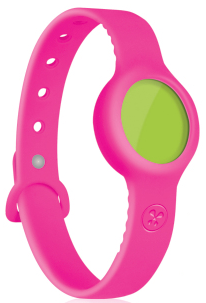
\includegraphics[scale=0.6]{figures/aProblemanalyse/nabi.png}
	\caption{På figuren ses Nabi Compete udformet som et armbånd. \citep{Perez2015}}
	\label{fig:nabi}
\end{figure}\vspace{-.25cm}
Der er muligt for børnene at konkurrerer individuelt, men hovedformålet er at konkurrere sammen med andre som et hold. Desuden kan børnene vælge en fødevare i brugerfladen, som kan informere børnene om, hvor meget fysisk aktivitet der kræves for at forbrænde denne fødevare. Herved kan der opstå konkurrence i at forbrænde flest kalorier eller løbe længst.\fxnote{Derudover lærer børnene om kalorier og distance ved at bruge appen, hvor det er muligt at følge med i progressionen.} Gennem konkurrencerne optjenes der point, som kan bruges til at købe et virtuelt dyr, der udvikles ved hjælp af point. \\
Dataet synkroniseres til en app gennem Bluetooth, hvor der kan gemmes data i op til 90 dage. Barnet og forældrene har dermed mulighed for at følge med i barnets progression. \\
Nabi Compete har endvidere en indkøbspris på 190 kr \citep{Fuhu2015,Fuhu_tech2015}.

\subsubsection{Vurdering af succeskriterier}
Aktivitetsmålerens funktioner vurderes ud fra opstillede succeskriterier i \secref{succeskrav}. \\
Aktivitetsmåleren detekterer gang og løb, men det er ikke muligt at skelne mellem aktivitetsformerne. Der detekteres heriblandt ikke cykling eller intensitet. Børnene aktiveres socialt, idet appen er designet med mulighed for at konkurrere mod hinanden eller arbejde sammen i hold. Derudover har børnene mulighed for %at have et kæledyr på appen, hvorved de, %udover at konkurrere mod andre, kan 
at se, hvor mange kalorier de har forbrændt. Aktivitetsmåleren er designet som et armbånd med en justerbar rem, hvilket gør at den kan monteres og placeres på komfortabel vis.~\citep{Fuhu2015,Fuhu_tech2015}\fxnote{Derudover er den designet således at den kan tåle sved og regn, hvilket gør at børnene kan bruge det i al slags vejr.}

Nabi Compete opfylder to ud af seks succeskriterier, mens det delvist opfylder to succeskriterier. En oversigt kan ses i \tabref{tab:sammenhold_tracker}.

\subsection{Ibitz}
Ibitz er en aktivitetsmåler, som henvender sig til børn over fem år gennem udfordringer i samarbejde med forældrene. Aktivitetsmåleren består af et pedometer, der måler skridt, og monteres ved en klemme, som det fremgår af~\figref{fig:ibitz}
\begin{figure}[H]
	\centering
	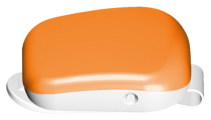
\includegraphics[scale=0.65]{figures/aProblemanalyse/ibitz.png}
	\caption{På figuren ses Ibitz, som benytts ved brug af klemmen. \citep{Ibitz_features2016}}
	\label{fig:ibitz}
\end{figure}\vspace{-.25cm}
Ibitz har generelle udfordringer inkorporeret og designet opfordrer til, at forældrene skal opsætte milepæle for barnet. Forældrene har mulighed for at udforme opgaver til deres barn, som de vurderer er passende i forhold til barnets fysiske aktivitetsniveau. Disse udfordringer kan indebære, hvor meget tid børnene skal bruge på en aktivitet. Ved at gennemføre udfordringerne, kan børnene optjene point, der kan bruges på to forskellige elektroniske spil. \newline 
Aktivitetsmåleren synkroniseres trådløst med en app via Bluetooth. Appen gemmer aktiviteterne i 30 dage, hvorved barnet og forældrene har mulighed for at følge med i progressionen.\\
Aktivitetsmåleren har endvidere en indkøbspris på 165 kr. \citep{Ibitz_features2016}

\subsubsection{Vurdering af succeskriterier}
Aktivitetsmålerens funktioner vurderes ud fra opstillede succeskriterier i \secref{succeskrav}. \\
Aktivitetsmåleren detekterer gang og løb men ikke cykling. Det er dog ikke muligt at skelne mellem aktivitetsformerne eller detektere intensitet. Børnene bliver delvist aktiveret socialt, hvor det primært er sammen med familien. Derudover aktiveres børnene ved at tjene point til forskellige spil, som oftest spilles sammen med andre børn. Aktivitetsmåleren monteres uden gene, da børnene selv kan vælge mellem at montere den på buksen eller skoen.\fxnote{Derudover kan den tåle vand, hvorved børn også kan bruge den i regnvejr}  

Ibitz opfylder to ud af seks succeskriterier, mens det delvist opfylder to succeskriterier. En oversigt kan ses i \tabref{tab:sammenhold_tracker}.

\subsection{Samlet vurdering af de udvalgte aktivitetsmålere}
Ovenstående analyse og vurdering af de udvalgte aktivitetsmålere viser, at ingen af aktivitetsmålere opfylder alle de opstillede succeskriterier fra \secref{succeskrav}. \newline
Fælles for aktivitetsmålerne er, at alle kan detektere løb og gang, men de kan ikke automatisk adskille disse aktivitetsformer. Yderligere er ingen af aktivitetsmålerne i stand til at detektere intensitet eller cykling. Det er vurderet, at alle aktivitetsmålerne har motiverende elementer således, at disse henvender sig til både fysisk aktive og inaktive børn. Desuden kan alle aktivitetsmålerne monteres og placeres på komfortabel vis, således børnene ikke oplever gener ved afbenyttelse. Resultatet af analysen fremgår i \tabref{tab:sammenhold_tracker}. %Indkøbsprisen for den enkelte aktivitetsmåler fremgår af nedenstående tabel. Denne pris vil kunne benyttes til at vurdere og sammenligne effektiviteten og prisen for de udvalgte aktivitetsmålere.  
\begin{table}[H]
	\centering
	\resizebox{\textwidth}{!}{%
		\begin{tabular}{l c c c c} \hline
			\rowcolor[HTML]{C0C0C0} 
			\multicolumn{1}{c}{\cellcolor[HTML]{C0C0C0}Krav} & \multicolumn{1}{c}{\cellcolor[HTML]{C0C0C0}Unicef Kid Power Band} & \multicolumn{1}{c}{\cellcolor[HTML]{C0C0C0}Sqord Booster}    &    \multicolumn{1}{c}{\cellcolor[HTML]{C0C0C0}Nabi Compete}     &   \multicolumn{1}{c}{\cellcolor[HTML]{C0C0C0}Ibitz} \\ \hline
			Detektere gang                                 & (x)                                        & (x)                                & (x)                               & (x)                        \\ \hline
			Detektere løb                                  & (x)                                        & (x)                                & (x)                               & (x)                        \\ \hline
			Detektere cykling                              &                                            &                                    &                                   &                            \\ \hline
			Detektere intensitet              &                                            &                                    &                                   &                            \\ \hline
			\begin{tabular}[c]{@{}l@{}}Motivere fysisk inaktive\\ såvel som fysisk aktive børn \end{tabular}         & x                                          & x                                  & x                                 & x                          \\ \hline
			Monteres uden gene                              & x                                          & x                                  & x                                 & x                          \\ \hline
			Pris                                 & 285 kr.                                        & 230 kr.                               & 190 kr.                               & 165 kr.                      \\ \hline
		\end{tabular}
	}
	\caption{I tabellen ses en oversigt over de fire udvalgte aktivitetsmålere, som er analyseret og vurderet på baggrund af deres respektive funktioner. (x) betyder, at de delvist lever op til succeskriterierne og x betyder, at de lever op til succeskriterierne.}
	\label{tab:sammenhold_tracker}
\end{table}\vspace{-0.5cm}
For at optimere de aktivitetsmålere, der benyttes i dag, vurderes det, at de skal være i stand til at adskille gang, løb og cykling. Barnet kan derved få overblik over dagens totale fysiske aktivitetsniveau. Derudover vurderes det som værende optimalt, hvis intensiteten af den fysiske aktivitet kan detekteres ved hjælp af puls. Denne er sigende for det fysiologiske udbytte af den givne aktivitet, hvilket beskrives i \secref{subsub:ak_int}.\newline
Aktivitetsmåleren skal aktivere børnene socialt sammen med andre børn. Derudover skal aktiviteterne foregå igennem leg eller spil, som både skal være baseret på konkurrence mod andre eller sammenspil i hold.